\section{The Complete Taxonomy}
Figure 1 shows the complete taxonomy proposed by this survey paper. 
It can be read similarly to a flowchart diagram. 
The way to apply it is after or during a read of some form of cyber detection literature perform the following steps. 
Start at the top left with the "Environment Defined?" decision block. Answer the yes or no question and follow the line for the answer. 
Each answer will lead to a block that says whether the literature made an explict statement about that particular category, or if you had to infer from context what subcategory to place the literature in. 
From whichever of those blocks selected, continue following the line to the subcategory box. 
Determine which subcategory from the list of choices presented in the box the literature falls under. 
In some cases, particularly in the data source, and detection method categories, there could be multiple that apply. 
Refer to previous figures for further refinement if there is interest. 
After applying a subcategory(s) continue to the green dot which will be the start of the dashed line leading to the next main category to classify the literature with. 
Continue this pattern until reaching the end of the categorization process.
It can be seen that for the detection method category the yes or no question is not if the authors define it.
This is because if the authors don't define a detection method at all then this taxonomy clearly doesnt apply and the literature doesnt fall under the subfield of cyber anomaly detection literature. 
Instead what is presented is a yes or no question about the method being a direct detection.

For subcategories that often have multiple instances for a single piece of literature, a cycle symbol is placed next to the subcategory box, to denote that you can return to that box multiple times before following the line to the end of the main category section. 
While only some of subcategories contain the multiple cycle symbol, there can potentially be multiple subcategories applied for any of the sections. 
However be careful in not over applying. For example if you reach the subcategory box for "anomaly type defined" and you think you can apply the sub category of all of them, then you should just choose APT. 
This is because, as noted before, APT groups make use of multiple types of attacks.
\begin{figure*}
  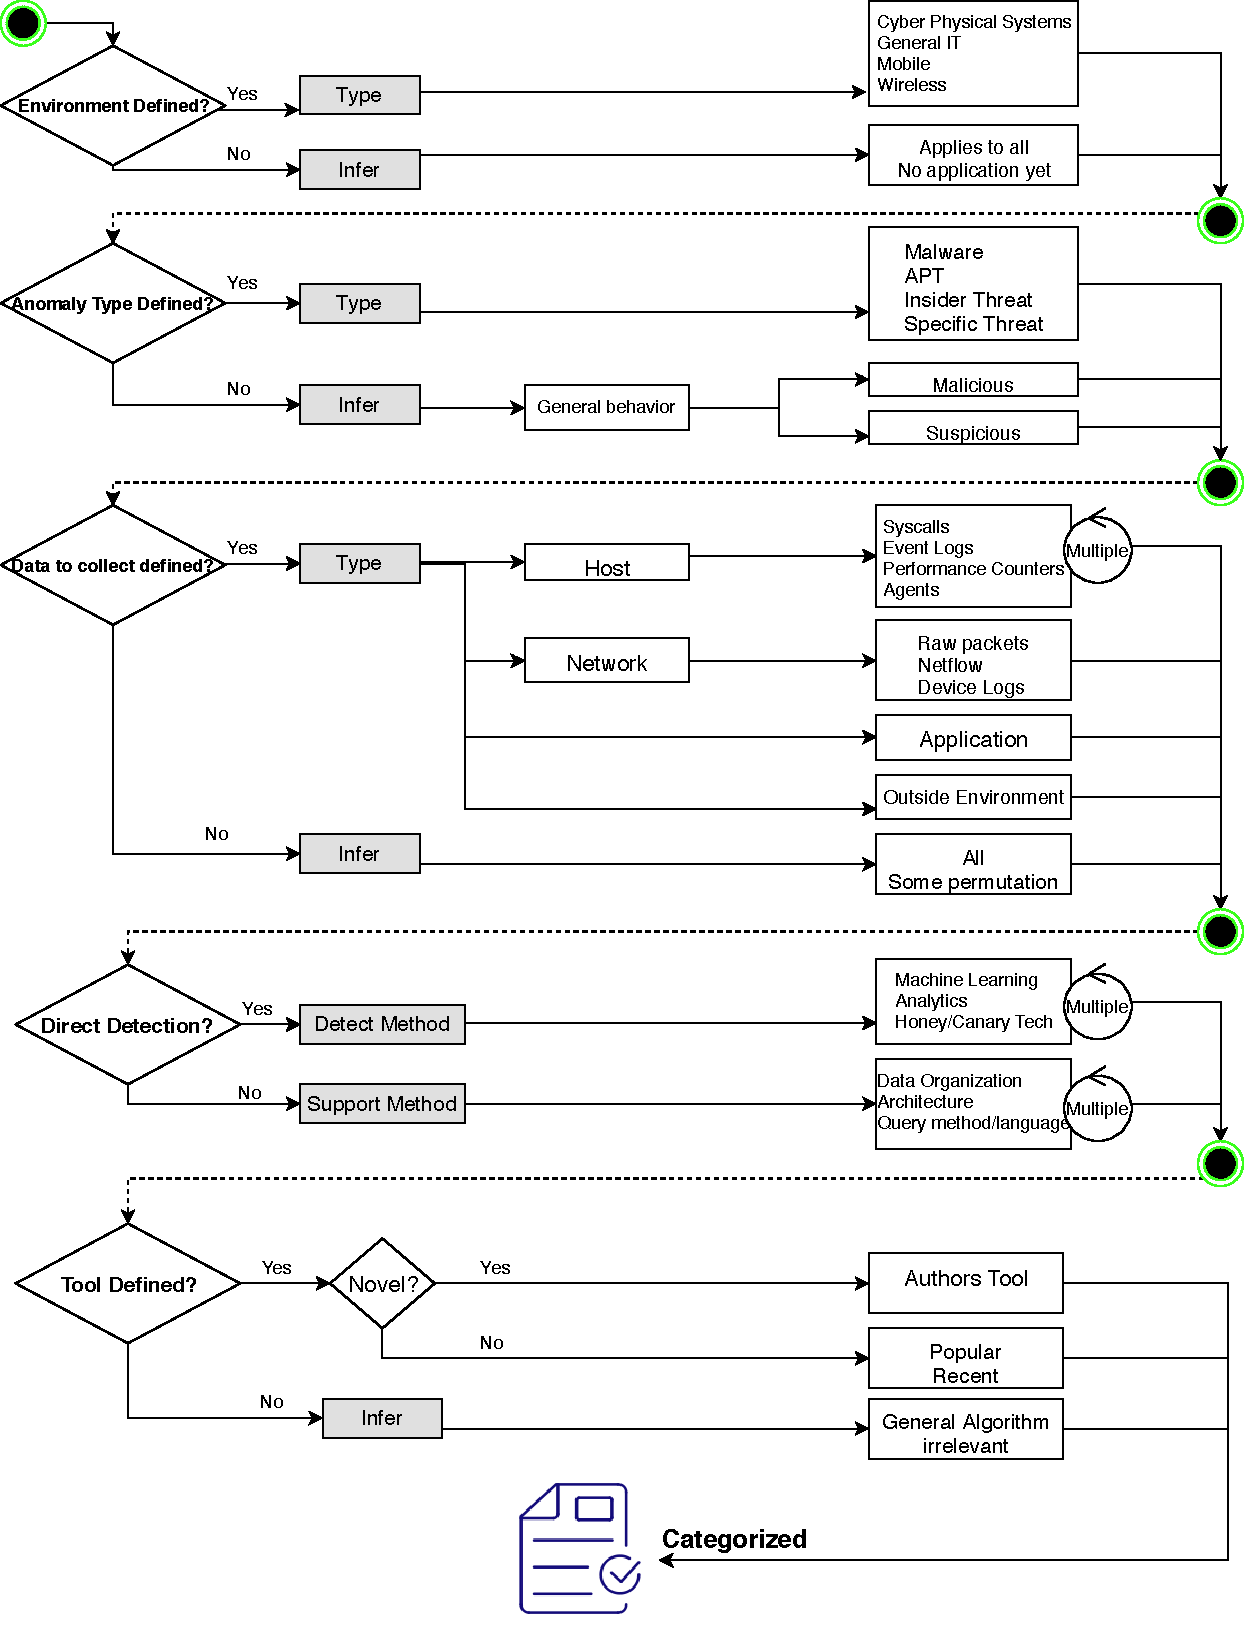
\includegraphics[width=\textwidth]{logicdiagram.pdf}
  \caption{Classification Model \yanyan{Please create a label, see below.}}
  \label{fig-model}
\end{figure*}